\pdfoutput=1
\documentclass[twocolumn]{aastex62}
%%\documentclass[]{emulateapj}

%Accepted/received/... %%

\received{xxx}
\revised{yyy}
\accepted{zzz}

%% Command to document which AAS Journal the manuscript was submitted to.
\submitjournal{AAS Journals}

%% Short title/authors

\shorttitle{LXUV History of TRAPPIST-1}
\shortauthors{Fleming et al.}

%% Begin document, title, packages %%
\usepackage{hyperref}
\usepackage{xspace}
\usepackage{graphicx}
\usepackage{amsmath}
\usepackage[caption=false]{subfig}

%% Custom commands
\def\mearth{{\rm\,M_\oplus}}
\def\rearth{{\rm\,R_\oplus}}
\def\msun{{\rm\,M_\odot}}
\def\rsun{{\rm\,R_\odot}}
\def\lsun{{\rm\,L_\odot}}
\def\gsim{~\rlap{$>$}{\lower 1.0ex\hbox{$\sim$}}}
\def\lsim{~\rlap{$<$}{\lower 1.0ex\hbox{$\sim$}}}

\newcommand{\xxx}[1]{{\textbf{#1}}}
\newcommand{\vplanet}[0]{\texttt{VPLanet}\xspace}
\newcommand{\approxposterior}[0]{\texttt{approxposterior}\xspace}
\newcommand{\eqtide}[0]{\texttt{EQTIDE}\xspace}
\newcommand{\stellar}[0]{\texttt{STELLAR}\xspace}
\newcommand{\kepler}[0]{\textit{Kepler}\xspace}

%% Begin doc %%
\begin{document}

\title{On The XUV Luminosity Evolution of TRAPPIST-1}

%% AUTHORS %%

%%\correspondingauthor{David P. Fleming}
%%\email{dflemin3@uw.edu}

%%\author[0000-0001-9293-4043]{David P. Fleming}
\author{David P. Fleming}
\affil{Astronomy Department, University of Washington \\
Box 951580, Seattle, WA 98195}
\affil{NASA Astrobiology Institute - Virtual Planetary Laboratory Lead Team, USA}

\author{Rory Barnes}
\affiliation{Astronomy Department, University of Washington \\
Box 951580, Seattle, WA 98195}
\affil{NASA Astrobiology Institute - Virtual Planetary Laboratory Lead Team, USA}

\author{Rodrigo Luger}
\affil{NASA Astrobiology Institute - Virtual Planetary Laboratory Lead Team, USA}
\affiliation{Center for Computational Astrophysics, Flatiron Institute \\
New York, NY 10010}

%% ABSTRACT %%

\begin{abstract}

Abstract.

- we constrain the stellar evolution and mass of TRAPPIST-1 using best priors and constraints currently available. we make our posterior distributions available for use with water loss simulations as the FXUV is a core input to such models, be it energy limited or recombination limited, maybe non-thermal escape models as well (look into that). our model and machine learning approach is all open source and documented on github, including a repo for the project itself
- TRAPPIST-1 conference stellar evolution stuff is 1st day, so email invited talks presenters and send them draft and thank them for their work which I use and cite in my own work - adam burgasser and jeff linsky
- 5 plots/tables: table of priors; corner plot; L, LXUV, R sampled from posteriors; \approxposterior comparison plot with distributions on top of each other 
- \citet{vanGrootel2018} decided luminosity and age were best constraints as R and Teff are unreliable for stellar models.  see their paper for a good discussion on this point and for good references to cite how metallicity or magnetic fields or incorrect opacity sources can lead to this discrepancy. See Filippazzo 2015 and Luger 2017 for additional age constraints to cite. Also from Burgasser 2017, "must be young based on the strength of its nonthermal magnetic emission (Bourrier et al. 2017; O’Malley-James Kaltenegger 2017"
- cite scholnik papers saying UV/Xray measurements of M dwarfs are critical, especially to estimate water losses and cite other HAZMAT papers for the activity evolution of M dwarfs
- note why I chose LXUV evolution as a function of time and not Rossby number, e.g. why I didn't use Wright+2018 data explicitely
- from Peacock+2018: "Late-type M stars remain UV active for much longer than their early M counterparts, typically with more variability in the FUV than the NUV (Miles Shkolnik 2017)."

\end{abstract}

%% Keywords %%

\keywords{}

%% Intro %%

\section{Introduction} \label{sec:intro}

"Although the dynamo processes that drive stellar activity and XUV emission in fully-convective stars have been shown to evolve qualitatively similar to solar-type stars \citep{Wright2016,Wright2018} ..."

Introduction about stellar activity for late type stars, what it is like and how late type stars evolve, and finally why it matters for exoplanet habitability, e.g. the XUV flux is a critical parameter for atmospheric escape and water loss, other loss mechanisms scale as FXUV to some power, like energy-limited and recombination-limited escape. In the intro, I explain what saturated and unsaturated phases correspond to physically, and under what conditions they are expected to occur. Argue how this qualitative behavior is observed for both partially and fully-convective stars, e.g. FGK and M dwarfs.

This study is critical and timely since people are modeling the hell out of TRAPPIST-1 and its planets and JWST proposals are going in to observe this system. My approach is generic and applicable to any systems with data and is relevant for LUVOIR where it can observe a statistically meaningful sample of planets, need \approxposterior for speed for constraints

\section{Model} \label{sec:model}

We simulate TRAPPIST-1's bolometric luminosity evolution using the \stellar module in \vplanet \citep{Barnes2016,vplanet2018} that performs a bicubic interpolation over mass and age of the \citet{Baraffe2015} stellar evolution tracks. The \citet{Baraffe2015} models, also employed by both \citet{Burgasser2017} and \citet{vanGrootel2018} to constrain TRAPPIST-1's stellar properties, were computed for solar metallicity stars and hence are valid for use with TRAPPIST-1, whose metallicity is consistent with solar \citep{Gillon2016}, although \citet{Burgasser2017} argue TRAPPIST-1 has a slightly super-solar metallicity based on isochrone modeling.

The L$_{X}$ evolution of fully convective stars has been shown to follow the same broken power law model examined for partially-convective low-mass FGK and M dwarfs \citep{Wright2016,Wright2018}. We therefore assume TRAPPIST-1's L$_{XUV}$ evolution traces that of L$_{X}$ and use the broken power law model of \citet{Pizzolato2003} and \citet{Ribas2005}:
\begin{align}
\label{eq:lxuv}
\frac{L_\mathrm{XUV}}{L_\mathrm{bol}} = \left\{
				\begin{array}{lcr}
					f_\mathrm{sat} &\ & t \leq t_\mathrm{sat} \\
					f_\mathrm{sat}\left(\frac{t}{t_\mathrm{sat}}\right)^{-\beta_\mathrm{XUV}} &\ & t > t_\mathrm{sat},
				\end{array}
				\right.
\end{align}
where $f_{sat}$ is ratio of stellar XUV to bolometric luminosity during the saturated phase, $t_{sat}$ is the duration of the saturated phase, and $\beta_{XUV}$ is the exponent that controls how steeply L$_{XUV}$ decays after saturation.

%% MCMC %%

\section{Markov Chain Monte Carlo} \label{sec:mcmc}

MCMC + constraints!

- we don't use radius or effective temperature or density constraints in our modeling for reasons explained in \citet{vanGrootel2018}
-\citet{Jackson2012} $f_{sat}$ measurements are derived for late K dwarfs through early F dwarfs, but are consistent with observations of fully-convective M dwarfs \citep{Wright2018}
- Jackson 2019 for M dwarf radius inflation

\subsection{Priors} \label{sec:mcmc:priors}

We leverage the extensive observations of TRAPPIST-1 and late M dwarfs to derive prior probability distributions for our MCMC analysis. We summarize our adopted prior distributions in Table~\ref{tab:priors} and justify our choices below. Following \citet{vanGrootel2018} who find that ... XXX. We adopt the age constraint for TRAPPIST-1 derived by by \citet{Burgasser2017}, age $\sim \mathcal{N}(7.6, 2.2^2)$, as their thorough analysis considered observations of TRAPPIST-1 and age indicators for peer systems. 

For low-mass stars in the saturated phase, the X-ray luminosity remains a constant fraction of the bolometric luminosity and is observed to cluster around $L_X/L_{bol} \approx -3$ \citep{Pizzolato2003,Wright2011,Wright2018} before decaying exponentially in the unsaturated regime. The saturation ratio shows tentative evidence of increasing with decreasing stellar mass \citep{Wright2011,Jackson2012}, consistent with the observation that later type low-mass stars are more active \citep[e.g.][]{West2008}. We assume the $L_{XUV}$ evolution traces that of $L_{X}$ and construct an empirical $f_{sat} = L_{XUV}/L_{bol}$ distribution from the sample of fully-convective, saturated stars with observed $L_{X}$ from \citet{Wright2011}. For each star in the sample, we follow \citet{Wheatley2017} and estimate $L_{XUV}$ as a function of L$_{X}$ using Eqn.~(2) from \citet{Chadney2015} and the stellar parameters given by \citet{Wright2011}. From the \citet{Wright2011} sample and our calculations, we find that the distribution of $L_{XUV}/L_{bol}$ for fully-convective M dwarfs in the saturated regime is well-approximated by a normal distribution with $f_{sat} \sim \mathcal{N}(-2.92, 0.26^2)$ and adopt it as our prior. 
 
The length of the saturated phase is estimated to be $t_{sat} \approx 100$ Myr for FGK stars \citep{Jackson2012}. Studies of L$_{XUV}$ evolution as a function of stellar age, or its proxy, rotation period, indicate that the activity lifetime, and hence duration of the saturated phase, is likely longer for later-type stars \citep{Shkolnik2014,Wright2011,GonzalezAlvarez2019}. Fully-convective M dwarfs can remain active for Gyrs, up to the ages of field stars \citep{West2008,Schneider2018}, with this trend persisting for slowly-rotating, and hence old, low-mass M dwarfs \citep{West2015}. TRAPPIST-1's high observed L$_{X}$ \citep{Wheatley2017}, short photometric rotation period \citep[3.3 d, ][]{Luger2017}, and Rossby number \citep[Ro $\approx 0.01$, ][]{Wright2018} suggest that TRAPPIST-1 is still saturated today \citep{Pizzolato2003,Wright2011,Wright2018,GonzalezAlvarez2019}. Both \citet{Roettenbacher2017} and \citet{Morris2018} suggest that the photometrically-determined rotation period might not be accurate, with the latter study showing that the 3.3 d period might correspond to a characteristic timescale for active regions on the stellar surface. Observations by \citet{Barnes2014} find $vsini = 6$ km s$^{-1}$ for TRAPPIST-1, corresponding to a rotation period of about 1 d for an inclination of $90^{\circ}$, implying that TRAPPIST-1's rapid rotation is likely physical.  Given these observational constraints, we adopt a broad uniform $t_{sat}$ prior distribution over $0.1 - 12$ Gyr.

In the unsaturated phase, L$_{X}$, and hence $L_{XUV}$, falls off exponentially with powerlaw slope $\beta_{XUV}$ \citep{Ribas2005}. \citet{Jackson2012} find that $\beta_{XUV}$ does not vary significantly with stellar mass in their sample of FGK stars, so we therefore adopt the distribution derived from their sample of late K dwarfs as our prior: $\beta_{XUV} \sim \mathcal{N}(-1.18, 0.31^2)$.

\begin{deluxetable}{lcc}
\tabletypesize{\small}
\tablecaption{Prior Distributions \label{tab:priors}}
\tablewidth{0pt}
\tablehead{
\colhead{Parameter} & \colhead{Prior} & \colhead{Notes}
}
\startdata
$m_\star$ [$M_{\odot}$] & $\mathcal{U}(0.07, 0.11)$ & Uniform \\  
$f_{sat}$ & $\mathcal{N}(-2.92, 0.26^2)$ & \citet{Wright2011},  \\
 &  & \citet{Chadney2015}  \\
$t_{sat}$ [Gyr] & $\mathcal{U}(0.1, 12)$ & Uniform \\
age [Gyr] & $\mathcal{N}(7.6, 2.2^2)$ & \citet{Burgasser2017} \\
$\beta_{XUV}$ & $\mathcal{N}(-1.18, 0.31^2)$ & \citet{Jackson2012}
\enddata \vspace*{0.1in}
\end{deluxetable}

%% Results %%

\section{Results} \label{sec:results}

Results.

\begin{figure*}[t]
\centering
	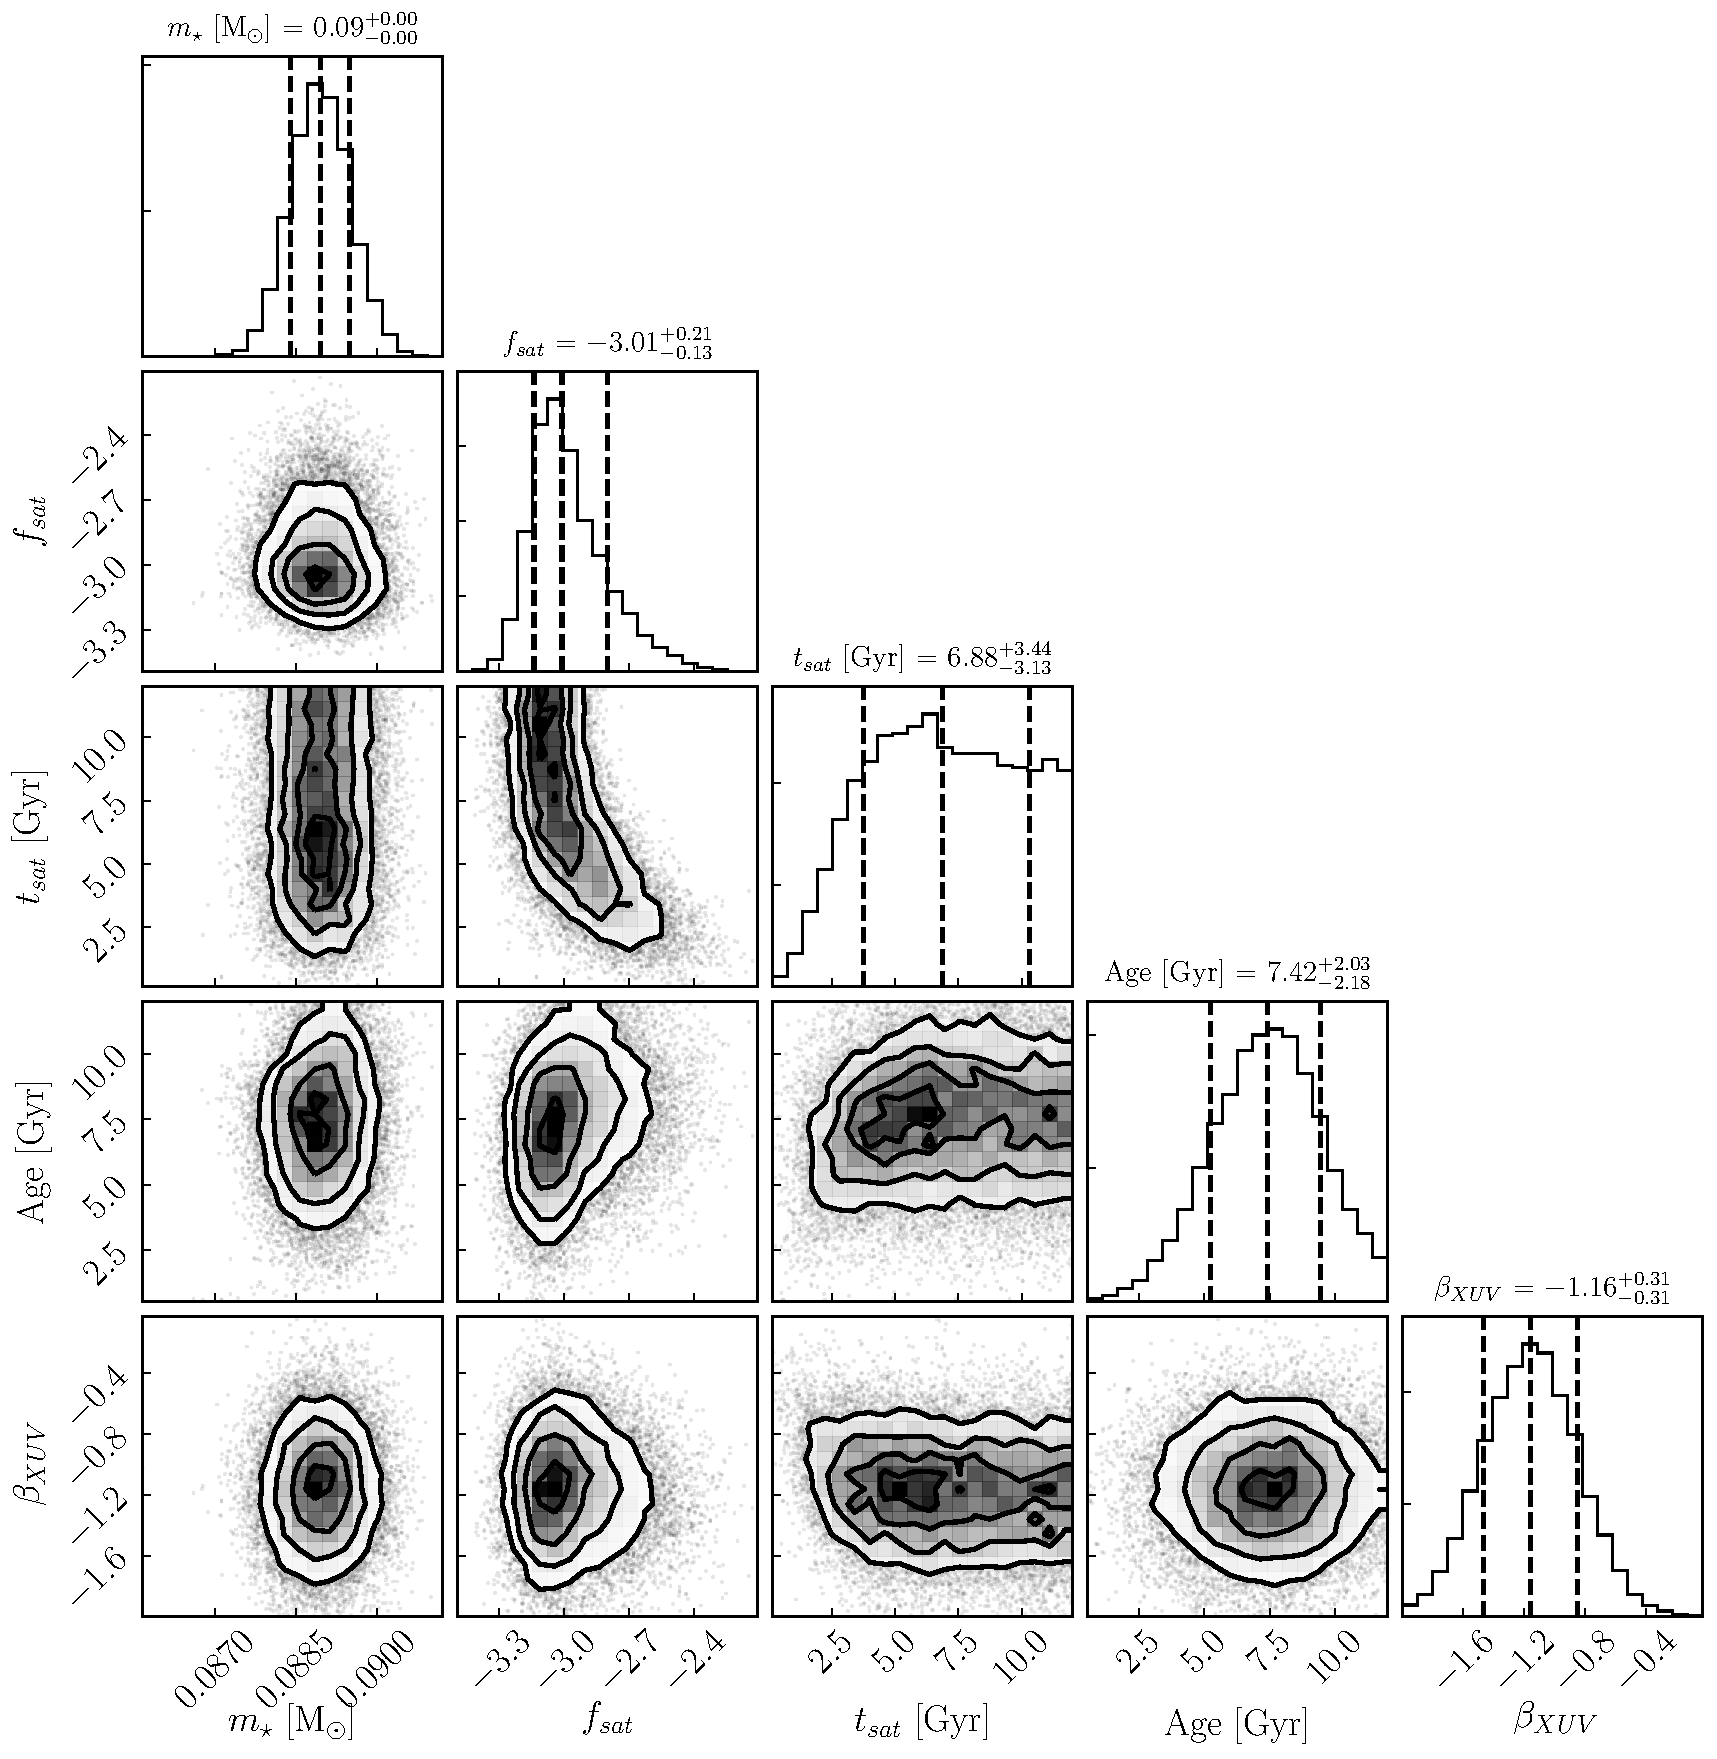
\includegraphics[width=0.75\textwidth]{../Analysis/Corner/trappist1Corner.pdf}
   \caption{Joint and marginal posterior probability distributions for the TRAPPIST-1 stellar parameters made using \texttt{corner} \citep{ForemanMackey2016}. From the posterior distribution, we infer that there is a $43.5\%$ chance that TRAPPIST-1 is still in the saturated phase today, i.e. P$(t_{sat} \geq \mathrm{ age } | \mathrm{data}) \approx 0.435$, and that there is only a $0.5\%$ chance that $t_{sat} \leq 1$ Gyr. Both the stellar age and $\beta_{XUV}$ mostly reflect the prior, although we find an age slightly lower, yet entirely consistent, with the age inferred by \citet{Burgasser2017}.}%
    \label{fig:corner}%
\end{figure*}


\begin{figure*}[t]
	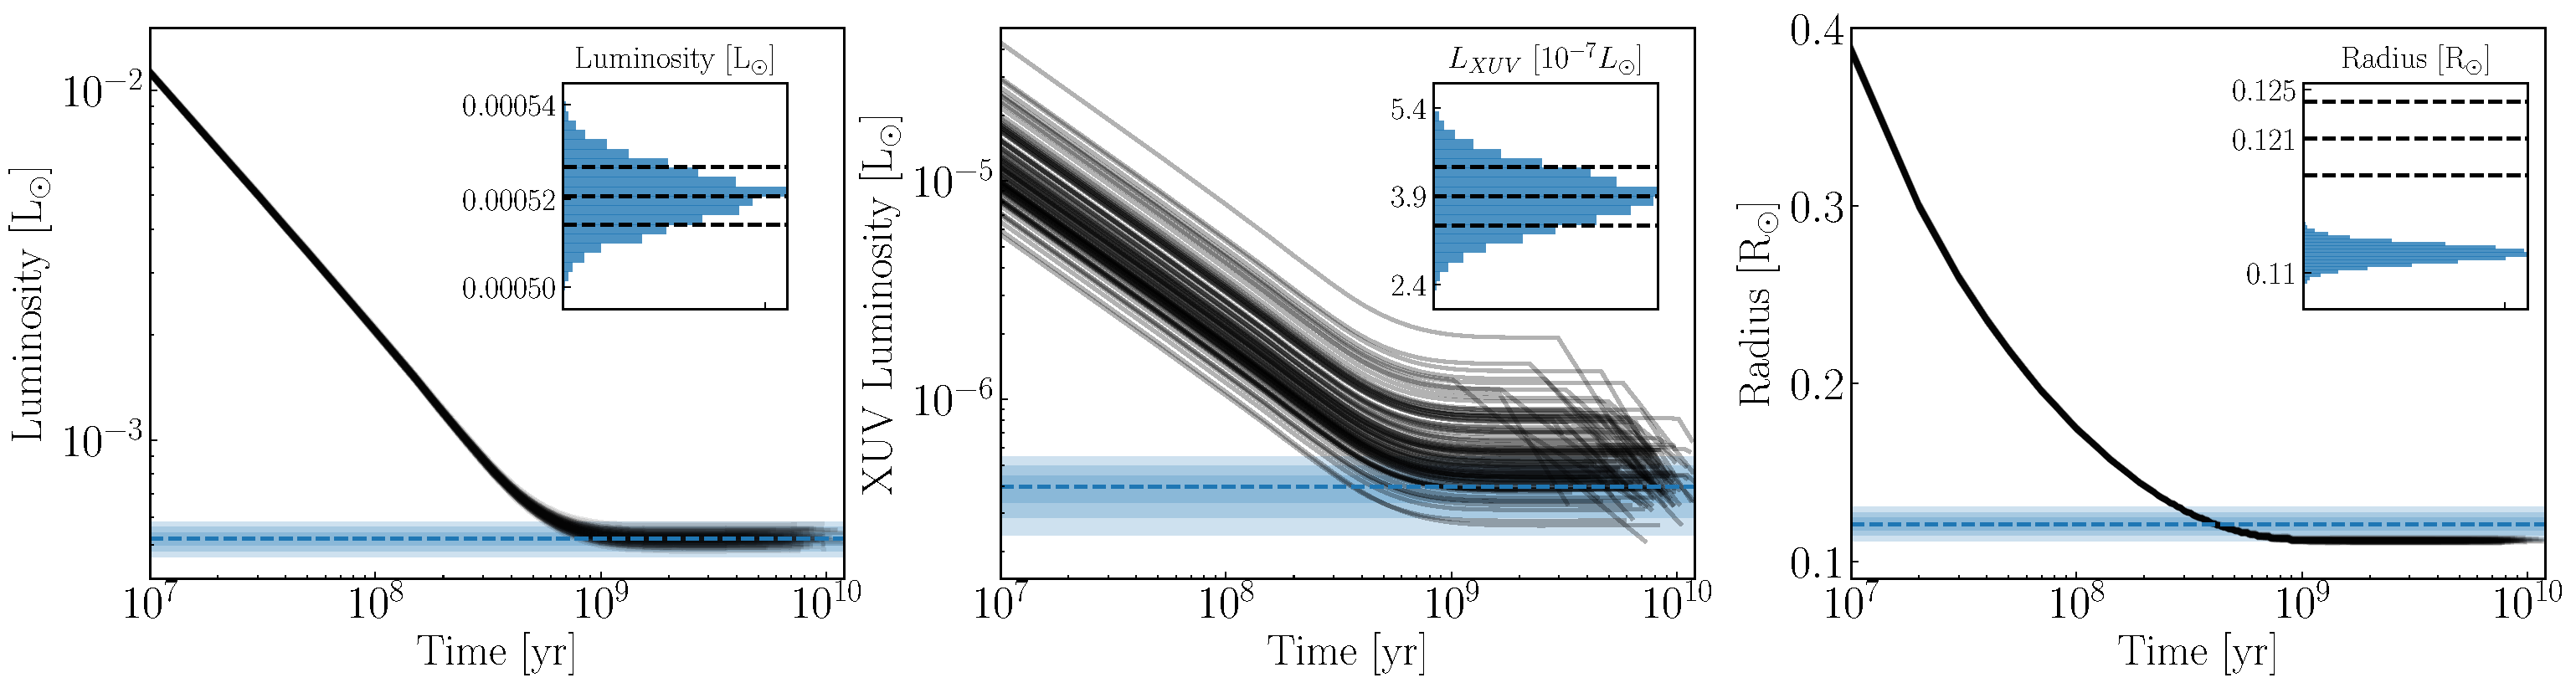
\includegraphics[width=\textwidth]{../Analysis/Evol/trappist1Evol.pdf}
   \caption{Plausible evolutionary histories of TRAPPIST-1's bolometric luminosity (left), XUV luminosity (center), and radius (right) simulated using \vplanet using 100 samples drawn from the posterior distribution. In each panel, the blue shaded regions display the 1, 2, and 3 $\sigma$ the observational uncertainties. The insets display the marginalized distributions of the quantities displayed in each panel evaluated at the age of the system, with the black dashed lines indicating the observed value and +/- 1 $\sigma$ uncertainty. The radius and bolometric luminosity constraints are adopted from \citet{vanGrootel2018}, and the L$_{XUV}$ constraint is taken from \citet{Wheatley2017}.}%
    \label{fig:evol}%
\end{figure*}

%% approxposterior %%

\section{\approxposterior} \label{sec:approx}

Results.

%% Discussion %%

\section{Discussion and Conclusions} \label{sec:discussion}

Discuss, and then conclude.

%% ACKNOWLEDGEMENTS %%
\acknowledgments
This work was facilitated though the use of advanced computational, storage, and networking infrastructure provided by the Hyak supercomputer system and funded by the Student Technology Fund at the University of Washington. DPF was supported by NASA Headquarters under the NASA Earth and Space Science Fellowship Program - Grant 80NSSC17K0482.  RB acknowledges support from the NASA Astrobiology Institute's Virtual Planetary Laboratory under Cooperative Agreement number NNA13AA93A.

%% SOFTWARE %%
\software{\approxposterior: \citet{FlemingVanderPlas2018}, \texttt{corner}: \citet{ForemanMackey2016}, \texttt{emcee}: \citet{ForemanMackey2013}, \texttt{matplotlib}: \citet{Hunter2007}, \texttt{numpy}: \citet{vanderWalt2011}, \vplanet: \citet{Barnes2016,vplanet2018}}, 

%% BIBLIOGRAPHY %%

\bibliography{trappist}

% End of file
\end{document}